\documentclass[tikz]{standalone}
%\usetikzlibrary{calc}
\usetikzlibrary{shapes,decorations}

\begin{document}

\tikzstyle{decision} = [diamond, draw, 
    text width=4.5em, text badly centered, node distance=3cm, inner sep=0pt]

% TRAFFIC LIGHT
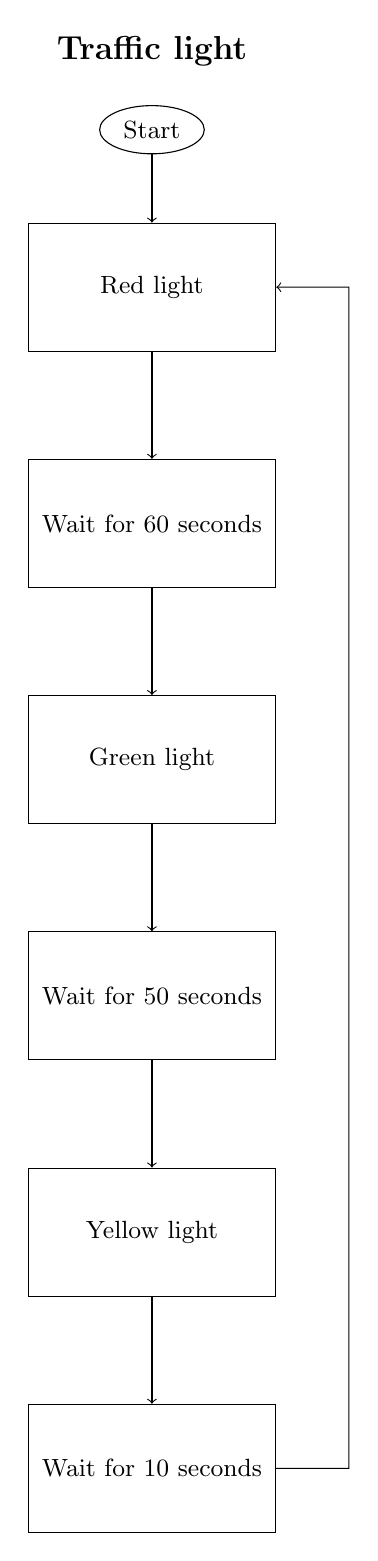
\begin{tikzpicture} [node distance=3cm, terminal/.style={ellipse, draw, text badly centered}, block/.style={rectangle, draw, text badly centered, minimum height=5em}]
{\small
	
	\node [terminal, ] (start1) {Start};
	\node [block, below of=start1, text width=9em, node distance=2cm] (light_1) {Red light};
	\node [block, below of=light_1, text width=9em, node distance=3cm] (light_2) {Wait for 60 seconds};
	\node [block, below of=light_2, text width=9em, node distance=3cm] (light_3) {Green light};
	\node [block, below of=light_3, text width=9em, node distance=3cm] (light_4) {Wait for 50 seconds};
	\node [block, below of=light_4, text width=9em, node distance=3cm] (light_5) {Yellow light};
	\node [block, below of=light_5, text width=9em, node distance=3cm] (light_6) {Wait for 10 seconds};
	
	% draw edges
	\draw [->] (start1) -- (light_1);
	\draw [->] (light_1) -- (light_2);
	\draw [->] (light_2) -- (light_3);
	\draw [->] (light_3) -- (light_4);
	\draw [->] (light_4) -- (light_5);
	\draw [->] (light_5) -- (light_6);
	\draw [->] (light_6) -- ++(2.5cm, 0) -- ++(0cm, 15cm) -- (light_1.east);
	
	% title
	\node[above of =start1,font=\large\bfseries,node distance=1cm] (title) {Traffic light};
}
\end{tikzpicture}

%% CAR GENERATOR
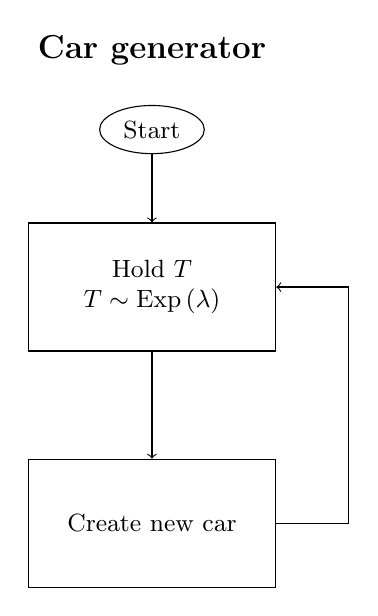
\begin{tikzpicture} [node distance=3cm, terminal/.style={ellipse, draw, text badly centered}, block/.style={rectangle, draw, text badly centered, minimum height=5em}]
{\small
	\node [terminal, ] (start2) {Start};
	\node [block, below of=start2, text width=9em, node distance=2cm] (cargen_1) {Hold $T$\\ $T \sim \mathrm{Exp}	\left(\lambda\right)$};
	\node [block, below of=cargen_1, text width=9em, node distance=3cm] (cargen_2) {Create new car};
	
	% draw edges
	\draw [->] (start2) -- (cargen_1);
	\draw [->] (cargen_1) -- (cargen_2);
	\draw [->] (cargen_2) -- ++(2.5cm, 0) -- ++(0cm, 3cm) -- (cargen_1.east);
	% title
	\node[above of =start2,font=\large\bfseries,node distance=1cm] (title) {Car generator};
}
\end{tikzpicture}


% CAR PROCESS iterative
\begin{tikzpicture} [node distance=3cm, terminal/.style={ellipse, draw, text badly centered}, block/.style={rectangle, draw, text badly centered, minimum height=5em}]
{\small
	\node [terminal, left of=start1, node distance=7.5cm] (start3) {Start};
	\node [block, below of=start3, text width=9em, node distance=2cm] (carproc_1) {Put car in queue};
	\node [decision, below of=carproc_1, text width=9em, node distance=3.5cm] (carproc_2) {Traffic light yellow or green?};
	\node [block, below of=carproc_2, text width=9em, node distance=3.5cm] (carproc_4) {Wait for 5 seconds};
	\node [block, left of=carproc_4, text width=9em, node distance=4.5cm] (carproc_3) {Remove from queue andDrive through};

	\node [terminal, left of=carproc_3, node distance=3cm] (stop3) {Stop};
	
	% draw edges	
	\draw [->] (start3) -- (carproc_1);
	\draw [->] (carproc_1) -- (carproc_2);
	\draw [->] (carproc_2.west) -- node [text width=1cm,midway,above,align=center ] {yes} (-12cm, -5.5cm)--(carproc_3.north);
	\draw [->] (carproc_2.south) -- node [text width=1cm,midway,right,align=center ] {no} (carproc_4.north);
	\draw [->] (carproc_4.east) -- ++(1cm,0) -- ++(0cm, 3.5cm) -- (carproc_2.east);
	\draw [->] (carproc_3) -- (stop3);
	
	% title
	\node[above of =start3,font=\large\bfseries,node distance=1cm] (title) {Car process};
}
\end{tikzpicture}

\begin{tikzpicture} [node distance=3cm, terminal/.style={ellipse, draw, text badly centered}, block/.style={rectangle, draw, text badly centered, minimum height=5em}]
{\small
	\node [terminal, left of=start1, node distance=7.5cm] (start3) {Start};
	\node [block, below of=start3, text width=9em, node distance=2cm] (carproc_1) {Put car in queue};
	\node [decision, below of=carproc_1, text width=9em, node distance=3.5cm] (carproc_2) {Traffic light yellow or green?};
	\node [block, below of=carproc_2, text width=9em, node distance=3.5cm] (carproc_4) {Passivate, \\ Wait for green light};
	\node [block, left of=carproc_4, text width=9em, node distance=4.5cm] (carproc_3) {Remove from queue and drive through};

	\node [terminal, left of=carproc_3, node distance=3cm] (stop3) {Stop};
	
	% draw edges	
	\draw [->] (start3) -- (carproc_1);
	\draw [->] (carproc_1) -- (carproc_2);
	\draw [->] (carproc_2.west) -- node [text width=1cm,midway,above,align=center ] {yes} (-12cm, -5.5cm)--(carproc_3.north);
	\draw [->] (carproc_2.south) -- node [text width=1cm,midway,right,align=center ] {no} (carproc_4.north);
	\draw [->] (carproc_4.south) -- ++(0,-1cm) -- ++(-4.5cm, 0) -- (carproc_3.south);
	\draw [->] (carproc_3) -- (stop3);
	
	% title
	\node[above of =start3,font=\large\bfseries,node distance=1cm] (title) {Car process};
}
\end{tikzpicture}

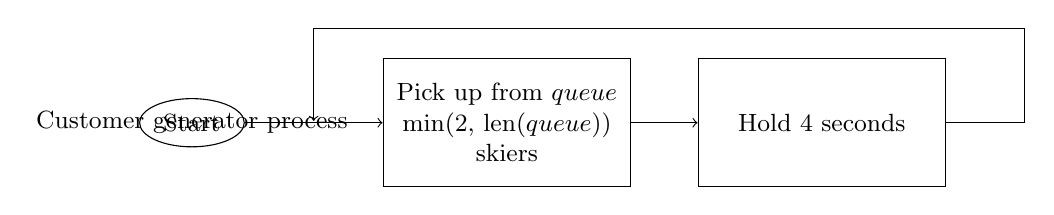
\begin{tikzpicture} [node distance=3cm, terminal/.style={ellipse, draw, text badly centered}, block/.style={rectangle, draw, text badly centered, minimum height=5em}]
{\small
  % Customer Generator
  \node (title) {Customer generator process};
  \node [terminal, ] (start) {Start};
  \node [block, right of=start, text width=9em, node distance=4cm] (pickup) {Pick up from $queue$ $\min (2,\, \mathrm{len}(queue))$ skiers};
  \node [block, right of=pickup, text width=9em, node distance=4cm] (wait) {Hold 4 seconds};
   Draw edges
  \draw [->] (start) -- node[midway,inner sep=0pt] (loop) {} (pickup);
  \draw [->] (pickup) -- (wait);
  \draw [->] (wait.east) -- ++(1cm, 0) -- ++(0cm, 1.2cm) -| (loop);
}
\end{tikzpicture}
\end{document}